\chapter{Locomotion Controller Transfer from the Virtual To the Real World}
\section{Motivation}
In character animation, we are able to reproduce many of the diverse and agile locomotion in nature. However, we have not yet seen the same level of motor capabilities in robotics. There is a large gap between what a character can do in the virtual environment and what a robot can do in the real world. This gap is due to the tremendous challenges when designing controllers with the real hardware since the majority of the robot controllers today are designed directly on the hardware. Robot hardware is expensive, has severe limitations (accuracy, repeatability, noise, torque limits, etc.), and requires frequent maintenance. For these reasons, designing robotic controllers is a time-consuming, labor intensive and trial-and-error process that is limited only to highly-specialized engineers. We have demonstrated in the previous chapters that with the powerful computational tools, controllers can be designed autonomously in a virtual environment. Can we extend the computational tools developed for character animations to \del{robotics to close the gap between these two fields?} \newtext{design  locomotion controllers for robots?}

The major challenge to directly apply the methods in character animation to robotics is the Reality Gap: Controllers that work effectively for a virtual character in the simulation may perform poorly on a robot in the real environment. The cause of the Reality Gap is the various simplifications in simulation algorithms, such as simplifying dynamics models, using inaccurate physical parameters, ignoring hardware limitations, noise and latency. For example, we do not model the internal mechanism of a servo in character animation. We often use rough estimations of the physical parameters, such as mass, COM and moment of inertia of a character in the simulation. Even though we can acquire some of these parameters from the Computer-Aided Design (CAD) specification files of a robot, they are also inaccurate given the manufacturing and assembling errors. Furthermore, we usually do not model the noise in the environment and the latency in the hardware communication in character animation.

\del{We need to cross the Reality Gap in order to tap the power of the computational tools to design robotic controllers autonomously.} \newtext{Although crossing the Reality Gap entirely is an extremely challenging problem, we can still tap into the power of the computational tools if we can sufficiently narrow down the differences between the simulation results and the real robot performance.} In this work, we develop a system with three components. In addition to physical simulation and controller optimization that we use extensively in character animation, we introduce \emph{simulation calibration} to narrow down the Reality Gap. During simulation calibration, we collect real performance data on the robot, and use it to improve our physical simulator. We optimize a set of simulation parameters to minimize the discrepancy between the simulation results and the collected real data. Through calibration, the simulator can capture the real world dynamics more faithfully. This calibrated simulator is used again in controller optimization to improve the quality of the controller. Depending on the task, a controller optimized in the simulation could be successfully transferred to a robot within a small number of iterations of simulation calibration and controller optimization. As a result, our system drastically reduces the number of time-consuming robot experiments and replaces the tedious manual tuning with an automatic optimization process. 

We evaluate our system using four locomotion tasks: rising from a leaning, sitting, or kneeling position to an erect stance, and flipping from a standing to a handstanding pose. These tasks play an important role in our daily life. They are so common that we perform them many times everyday. Although most of us can achieve these tasks without difficulties, they present big challenges for some elderly persons and patients with hamstring injuries. We choose to study these motions and synthesize them on a robot, given its important health-care applications. One simple solution to achieve these tasks is to utilize static balance. The robot can increase the area of the support polygon by establishing new contact points, and then raise its body slowly while maintaining the COM within the support polygon. We choose not to use this strategy because in real life, we humans can perform these motions in a more agile fashion, and we hope that our controller can demonstrate comparable agility. For this reason, our controllers will utilize impulsive actions and take advantage of the accumulated momentum to rise. In addition, since the main contribution of our method is simulation calibration, to best test its effectiveness, we only use feedforward controllers in our evaluations. Otherwise, if feedback controllers are used, the stability region of the tasks could be drastically increased, which makes the simulation accuracy less critical. Our results show that simulation calibration is \del{an effective method for crossing the Reality Gap.} \newtext{effective to transfer the controllers from the virtual to the real environments for certain locomotion tasks.} In all the test cases, at most two iterations of calibration is needed before the controllers work on the real robot.

\section{Overview}

\begin{figure}[!t]
  \centering
  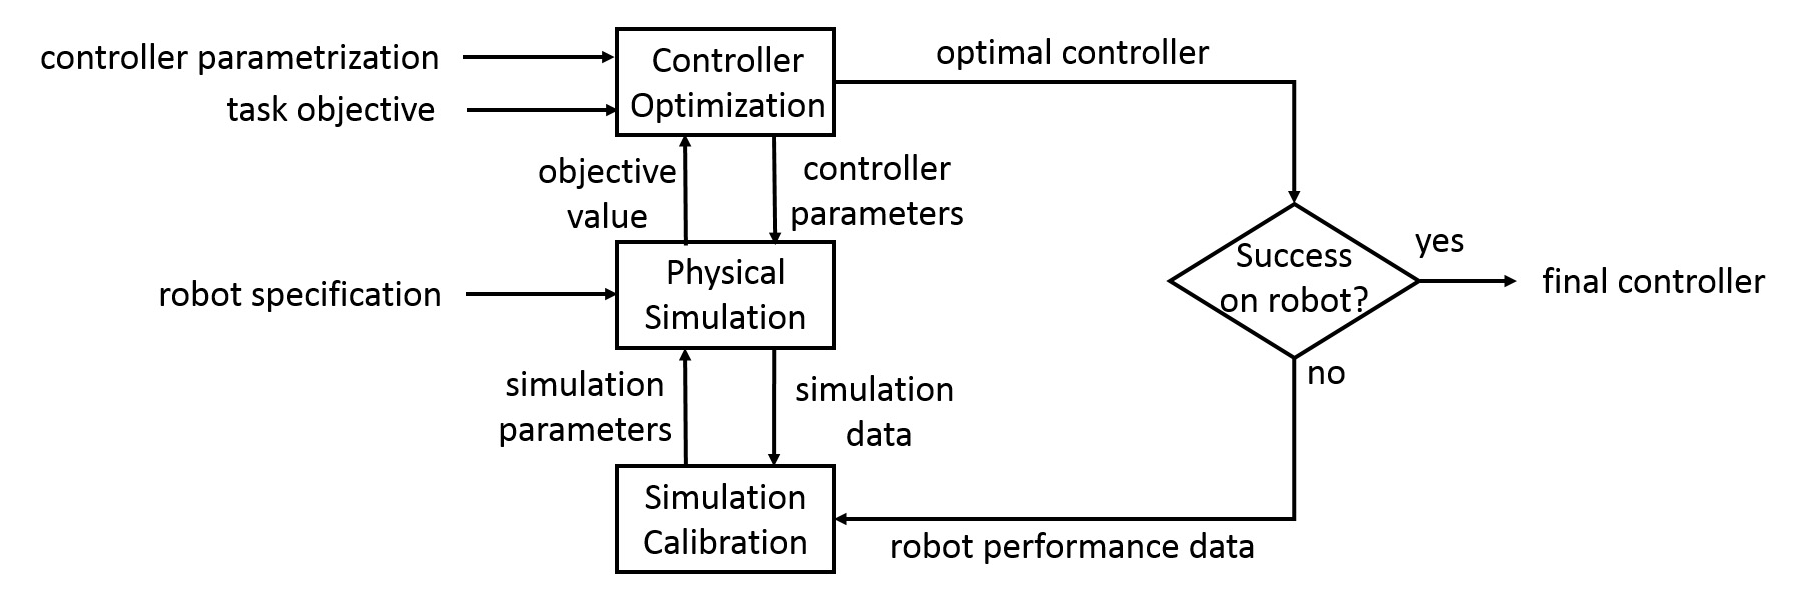
\includegraphics[width=6in]{figures/controllerTransfer}
  \caption{Overview of our algorithm.}
  \label{fig:controllerTransferOverview}
\end{figure}

We have developed a system that can automatically design locomotion controllers for robots (Figure~\ref{fig:controllerTransferOverview}). Given the specification of the robot, including its body shape, the physical properties of each body, and the types of joints, we build a physical simulation using Dynamic Animation and Robotics Toolkit (DART) \cite{dart:2012}. In addition, we also incorporate into the simulation the torque limits, servo models and communication latency, which are often omitted in character animation. The controller optimization subsystem runs thousands of simulations to search for the optimal controller that maximizes the task-related fitness function. We then test this optimal controller on the robot. If the robot successfully completes the task, a working robotic controller is found and our algorithm terminates. Otherwise, we record the robot performance data and feed it into the simulation calibration subsystem. Simulation calibration runs another optimization, which searches for the optimal simulation parameters to minimize the discrepancy between the performance of the robot in the simulation and in the real world. The loop of controller optimization and simulation calibration is performed iteratively until the controller works successfully on the real robot. In the next three sections, we will present the algorithmic details of these components.

\section{Physical Simulation}

\subsection{Dynamics Equations}

We model the robot as an articulated rigid body system in our simulator. We represent the states of the system $(\mathbf{x}, \dot{\mathbf{x}})$ in generalized coordinates, where $\mathbf{x}$ includes the global position $\mathbf{p}$, the orientation $\mathbf{r}$ of the root link, and the joint angles $\mathbf{q}$. We solve the governing equations of motion in generalized coordinates:

\begin{equation}
\label{eq:robotdynamics}
\mathbf{M}(\mathbf{x})\mathbf{\ddot{x}}+\mathbf{C}(\mathbf{x},\mathbf{\dot{x}})=\mathbf{\tau}+\mathbf{J}^T\mathbf{f}
\end{equation}
where $\mathbf{M}(\mathbf{x})$ is the mass matrix and $\mathbf{C}(\mathbf{x},\mathbf{\dot{x}})$ is the Coriolis and Centrifugal force. $\mathbf{\tau}$ are joint torques exerted by the actuators. $\mathbf{J}$ is the Jacobian matrix and $\mathbf{f}$ is the external contact force, which is computed based on linear complementarity conditions. In our implementation, we use DART to compute the contact force and numerically integrate the system state $(\mathbf{x}, \dot{\mathbf{x}})$ over time.

\subsection{Actuator Model}
\label{sec:motorDynamics}
In character animation, the joint torque $\tau$ is often chosen as the control signal since the torques can be directly integrated in eq.(\ref{eq:robotdynamics}). However, the control signal for the robot that we use in the experiments is the desired joint angles $\bar{\mathbf{q}}$. Given the difference between the desired and the current angle ${q-\bar{q}}$ of each joint, the servo first maps it to a corresponding power level $U$ that is equivalent to changing the voltage across the motor and the voltage is eventually converted to the joint torque $\tau$ according to the internal actuator dynamics.

\begin{figure}[t]
\centering
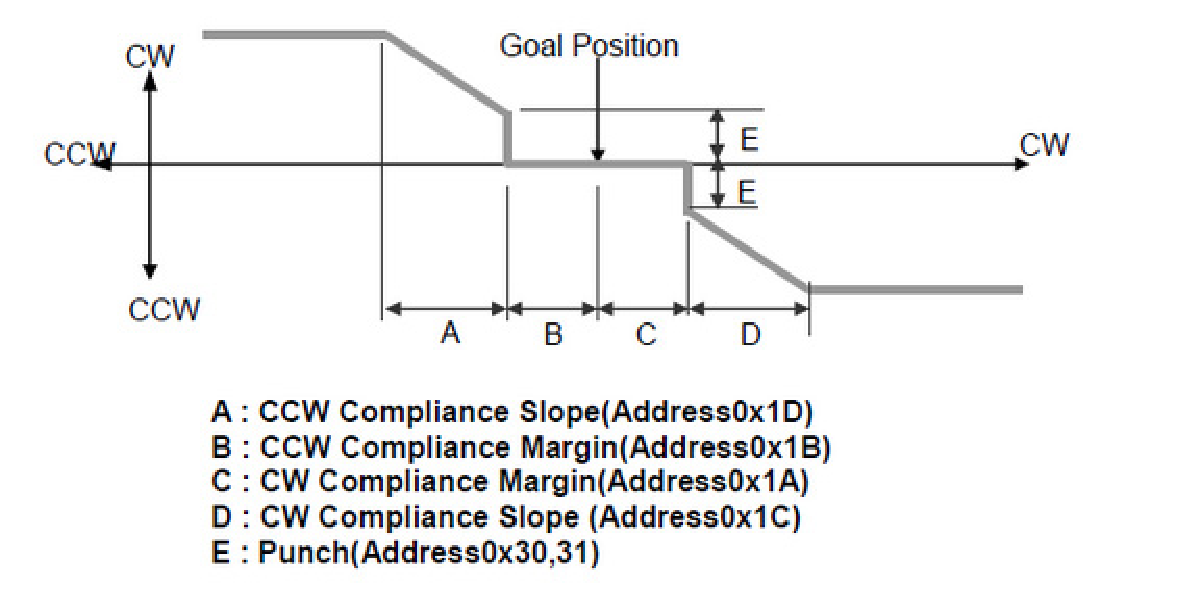
\includegraphics[width=5in]{figures/ax18gain.eps}
\caption{The mapping between $q-\bar{q}$ and $U$ for an AX-18 actuator. This figure is from the user manual of Dynamixel AX-18 Actuator \cite{AX18:2015}. The x-axis is $q-\bar{q}$ while the y-axis is $U$.}
\label{fig:actuatorMap}
\end{figure}

We choose BIOLOID GP as our robot platform. BIOLOID GP is a humanoid robot that consists of 18 degrees of freedom powered by Dynamixel AX-12/AX-18 servos. All the actuators on the lower body of the robot are Dynamixel AX-18, which use the following mapping (Figure \ref{fig:actuatorMap}) between the joint angle difference $q-\bar{q}$ and the power level $U$. The intervals A and D determine the slope of the actuator response for counter-clockwise and clockwise motions respectively. Smaller values mean steeper response slopes, in which case the actuator follows the desired angle more closely. However, too small a value can lead to overshooting problems. B and C are the compliance margins. If the error of angle is within a small margin specified by B and C, the servo does not output any torque. E, the punch, is the minimum power level before the servo shuts down. In practice, we set A and D to be the same so that the simulated servo will behave the same no matter it rotates clockwise or counter-clockwise. In addition, since B, C and E are very small compared to A and D, we ignore their effects and approximate the mapping as linear within the intervals $q-\bar{q}\in A\bigcup B\bigcup C\bigcup D$ with the slope $k_e$:
\begin{equation}
  U=k_e(q-\bar{q})
  \label{eqn:voltageErrorRelation}
\end{equation}

To derive the relation between the power level $U$ and the output torque $\tau$, we adopt a model for the ideal DC motor \cite{SchwarzB:2013}. It is valid to assume an ideal model because the AX-18 servos use high-quality DC motors. The derivation follows by considering the power balance in the motor at a constant voltage U:
\begin{equation}
  P_{electric} = P_{mechanic} + P_{heat}
  \label{eqn:powerBalance}
\end{equation}
where $P_{electric}$ is the electrical power, $P_{mechanic}$ is the mechanical power, and $P_{heat}$ is the power dissipated as heat. From eq.(\ref{eqn:powerBalance}), we can get the following relation:
\begin{equation}
UI=\dot{q}\tau_{motor} + RI^2
\end{equation}
where $I$ is the current and $R$ is the motor winding resistance. In an ideal DC motor, the torque is linearly proportional to the current $\tau_{motor}=k_{\tau}I$. Plugging it into the above equation, we arrive at the relation between the voltage $U$ and the total torque generated by the motor $\tau_{motor}$:
\begin{equation}
  U=k_{\tau}\dot{q}+\frac{R}{k_{\tau}}\tau_{motor}
  \label{eqn:votageTorqueRelation}
\end{equation}
where $k_{\tau}$ is the torque constant, which is determined by the hardware design of the motor. The total torque generated by the motor is not yet the output torque that drives the motor shaft due to the friction inside the motor. The total torque can be decomposed into the output torque $\tau$ and the friction torque $\tau_f$.
\begin{equation}
  \tau_{motor}=\tau+\tau_f
  \label{eqn:torqueBalance}
\end{equation}
The friction torque can be further divided into viscous friction and Coulomb friction \cite{SchwarzB:2013}:
\begin{equation}
  \tau_f = k_v\dot{q}+k_c\sgn(\dot{q})
  \label{eqn:frictionComponents}
\end{equation}
where $k_v$ and $k_c$ are friction coefficients for the viscous and Coulomb friction respectively. $\sgn(x)$ is the sign function that equals 1 if $x$ is positive, -1 if $x$ is negative and 0 otherwise.

Combining eq.(\ref{eqn:votageTorqueRelation}), (\ref{eqn:torqueBalance}) and (\ref{eqn:frictionComponents}), we get the relation between the error of the joint angle $q-\bar{q}$ and the output torque $\tau$.
\begin{align}
\nonumber  \tau & = \frac{k_{\tau}k_e}{R}(q-\bar{q})+(-k_v-\frac{k_{\tau}^2}{R})\dot{q}-k_c\sgn(\dot{q})\\
\nonumber & = -k_p(q-\bar{q}) - k_d\dot{q} - k_c\sgn(\dot{q})\\
  \label{eqn:torqueErrorRelationSimple}
\end{align}
where $k_p=-\frac{k_{\tau}k_e}{R}$ and $k_d=k_v+\frac{k_{\tau}^2}{R}$. We call these values $k_p$, $k_d$ and $k_c$ the \emph{actuator gains}. It is possible to compute these actuator gains if the related parameters are given in the specification sheet of the motor. Plugging eq.(\ref{eqn:torqueErrorRelationSimple}) into (\ref{eq:robotdynamics}), and taking torque limits $[\tau_{min}, \tau_{max}]$ into consideration, we get the dynamics equation that use the desired joint angles as the control signal.
\begin{displaymath}
 \mathbf{M}(\mathbf{x})\mathbf{\ddot{x}}+\mathbf{C}(\mathbf{x},\mathbf{\dot{x}}) = \tau+\mathbf{J}^T\mathbf{f} \\
  \end{displaymath}
where 
\begin{displaymath}\tau =
  \left\{
    \begin{array}{ll}
      \tau_{min} & \text{if }\tau < \tau_{min},\\
      \tau_{max} & \text{if }\tau > \tau_{max},\\
      -k_p(\mathbf{q}-\bar{\mathbf{q}}) - k_d\dot{\mathbf{q}} - k_c\sgn(\dot{\mathbf{q}}) & \text{otherwise.}\\
    \end{array}
  \right.
  \label{eqn:robotDynamicsControl}
\end{displaymath}

\paragraph{Actuator Gain Identification.} We design robot experiments to identify the actuator gains $k_p$, $k_d$ and $k_c$, since the specification of the servos does not provide the necessary information to compute them. In the experiment, we clamp the entire robot on a table except for the left foot. We then send a periodic control signal $\bar{q}(t)$ to the servo at the left ankle (blue curve in Figure \ref{fig:actuatorId} Left). The desired joint angle stays at the maximum value for 0.67 second, then changes to the minimum value and stays for another 0.67 second and repeats. We record the trajectory of the actual joint angle $q(t)$ through the experiment (green curve in Figure \ref{fig:actuatorId} Left). We manually segment out portions of these two curves where the power level is approximately linear to the error $\Delta q = q-\bar{q}$ (the union of intervals A, B, C and D in Figure \ref{fig:actuatorMap}). The black ``+'' in Figure~\ref{fig:actuatorId} Right shows this error over time $\Delta q(t)$ in a typical segment.

\begin{figure}[!t]
  \centering
  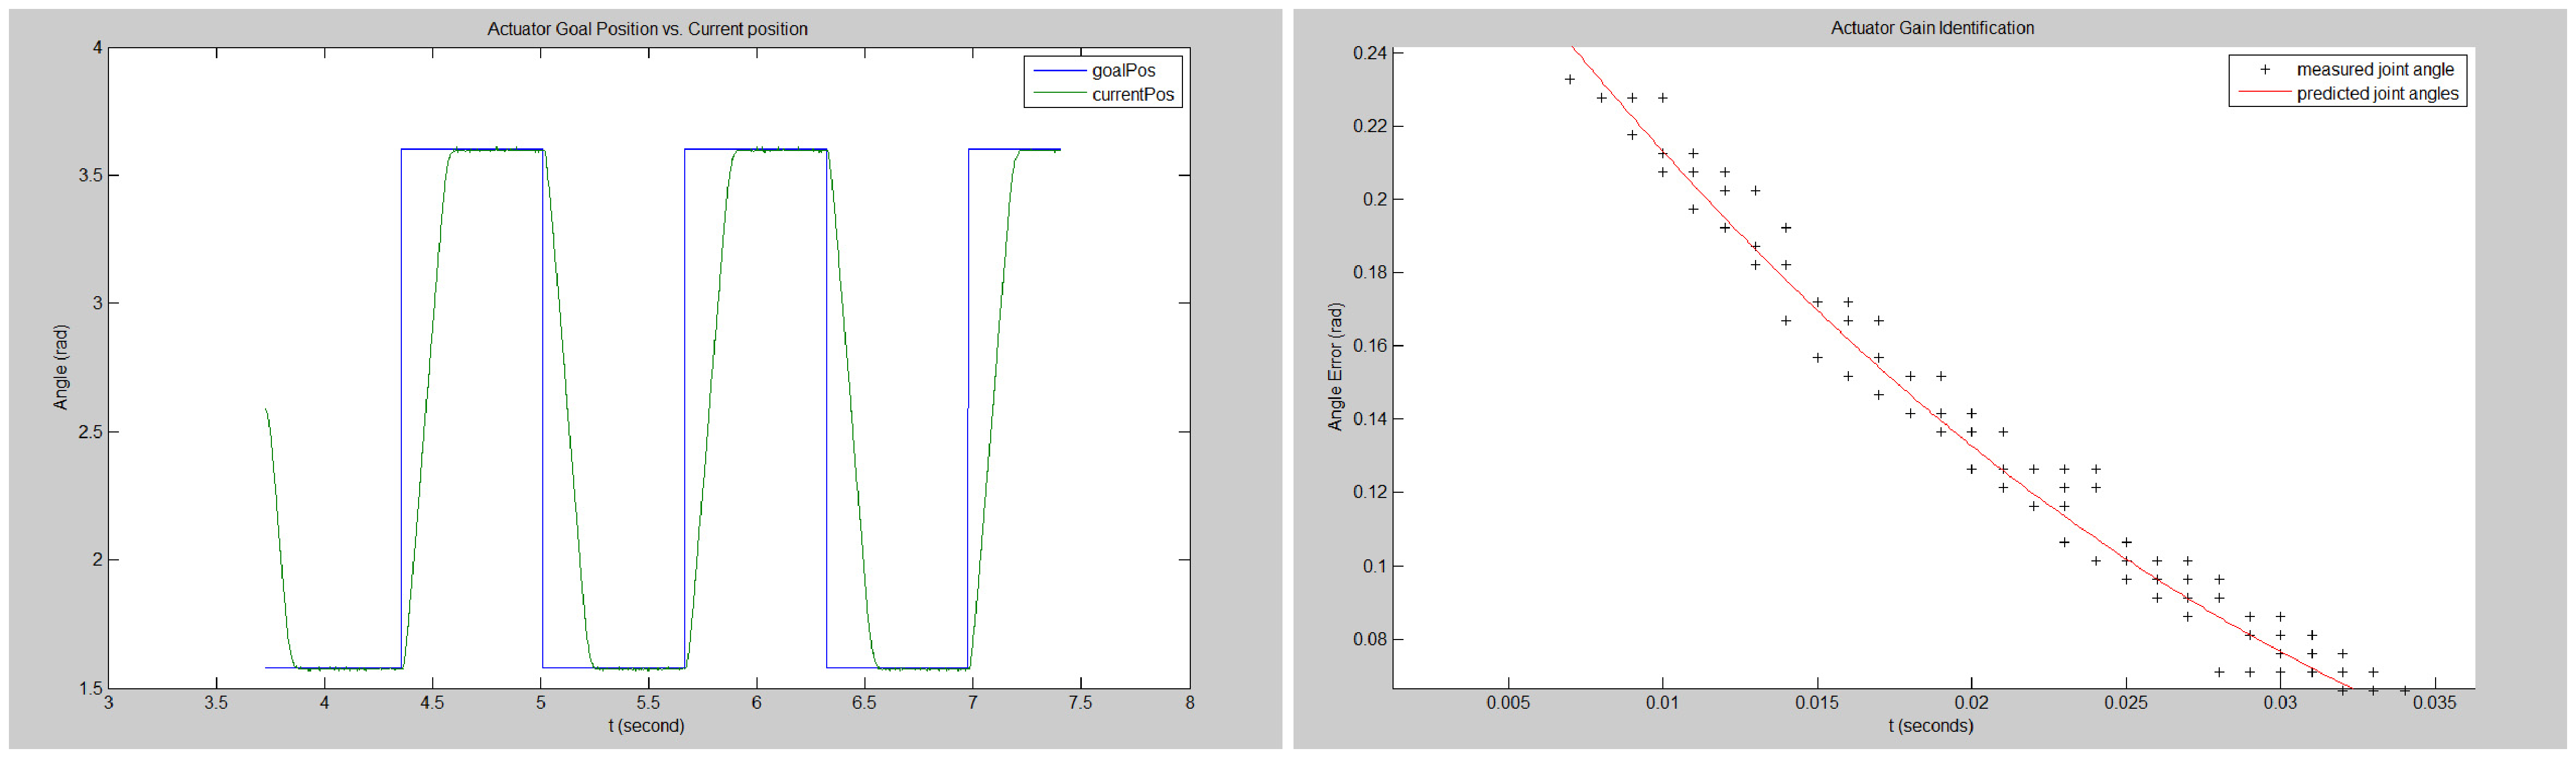
\includegraphics[width=\textwidth]{figures/actuatorId}
  \caption{Actuator Identification. Left: the time series of input desired joint angle and the measured joint angle for an AX-18 servo. Right: the time series of actual error of joint angle and the predicted error using the identified actuator gains.  }
  \label{fig:actuatorId}
\end{figure}

Given $q(t)$ and $\bar{q}(t)$, we can apply regression to estimate the actuator gains. From eq. (\ref{eqn:torqueErrorRelationSimple}), we have
\begin{equation}
\ddot{q}=I^{-1}(-k_p\Delta q - k_d\dot{q} - k_c\sgn(\dot{q}))
\end{equation}
where $I$ is the moment of inertia of the foot with respect to the rotating axis. The above equation is derived by plugging into $\tau = I\ddot{q}+\dot{I}\dot{q}$ and the fact that $\dot{I}\dot{q}=0$ because the foot is a rigid body that rotates along a fixed axis. Ideally, $\ddot{q}$ and $\dot{q}$ can be computed using finite difference. However, the measurement of $q(t)$ is too noisy and finite difference would greatly magnify the noise. To solve this problem, we first smooth $q(t)$ by performing a 4th-order polynomial regression:
\begin{equation}
  \min_{a,b,c,d,e}\int ||q(t)-(at^4+bt^3+ct^2+dt+e)||^2\mathrm{d}t
  \label{eqn:Deltaq}
\end{equation}
where $a,b,c,d,e$ are the polynomial coefficients. This regression gives us a smooth analytical expression of $q(t)$. We then compute $\ddot{q}$ and $\dot{q}$ by differentiate this polynomial analytically:
\begin{align}
\label{eqn:Deltaqdot}  \dot{q}(t)&=4at^3+3bt^2+2ct+d\\
\label{eqn:Deltaqddot}  \ddot{q}(t)&=12at^2+6bt+2c
\end{align}

Combining eq. (\ref{eqn:Deltaq}), (\ref{eqn:Deltaqdot}) and (\ref{eqn:Deltaqddot}), we can perform another regression to compute the actuator gains.
\begin{equation}
\min_{k_p, k_d, k_c}\int||\ddot{q}(t)-I^{-1}(-k_p(q(t)-\bar{q}(t)) - k_d\dot{q}(t) - k_c\sgn(\dot{q}(t)))||^2\mathrm{d}t
\end{equation}

Our experiments and computation show that the actuator gains are $k_p=9.272(N\cdot m/rad)$, $k_d=0.3069(N\cdot m\cdot s/rad)$, and $k_c=0.03(N\cdot m)$. To verify the correctness of these values, we plug them into the simulator and repeat the same experiment in the simulation. The red curve in Figure \ref{fig:actuatorId} Right is the error over time predicted in our simulation, which agrees well with the data that was collected from the robot experiment.

\paragraph{Latency.} To guarantee the stability of the simulation, we use 1ms as the simulation time step. Many animation systems use the same simulation and control frequency, which means that a control signal $\bar{\mathbf{q}}$ is updated every simulation time step. However, the average latency of the whole control loop on our robot is 16ms. It is measured by a timer in our program between the time that the program starts sending the actuator commands to the robot and the time that it finishes reading the sensor measurements from the robot. To better match our simulation with the actual latency, we choose to only update the control signal every 16 time steps.

\section{Controller Optimization}

Given the physical simulation, we can design controllers to enable the robot to achieve various locomotion tasks in the simulated environment. The four tasks that we use to test our system are rising from a leaning, sitting or kneeling position to an erect stance, and flipping from a standing to a handstanding pose. For each task, the joint configuration of the initial pose and the final pose are provided by the user. The goal of controller optimization is to find a sequence of control signals $\bar{q}(t)$ so that the robot can move from the initial to the final pose without losing balance. We purposefully choose to use only feedforward controllers\footnote{There is still an internal feedback loop in the actuators to track the desired joint angle (See Chapter~\ref{sec:motorDynamics}). However, this feedback loop is not fully programmable.} in this work, which means that the control signal $\bar{\mathbf{q}}(t)$ is a only function of time $t$ and does not depend on the states of the robot. With the feedforward control alone, the controller transfer can only succeed if the simulation is close enough to the real-world environment. This will put the simulation calibration subsystem into more thorough tests.

We first formulate a trajectory optimization problem for each task.
\begin{align}
 \label{eqn:obj}&\max_{\bar{\mathbf{q}}(t),T} V_{ctrl}(\mathbf{x}(t))\\
\nonumber  \mathrm{subject\;} &\mathrm{to} \\
\label{eqn:dyn1} & \mathbf{M}(\mathbf{x})\mathbf{\ddot{x}}+\mathbf{C}(\mathbf{x},\mathbf{\dot{x}}) =\tau + \mathbf{J}^T\mathbf{f}\\
\label{eqn:dyn2} &\tau =
  \left\{
    \begin{array}{ll}
      \tau_{min} & \text{if }\tau < \tau_{min},\\
      \tau_{max} & \text{if }\tau > \tau_{max},\\
      -k_p(\mathbf{q}-\bar{\mathbf{q}}) - k_d\dot{\mathbf{q}} - k_c\sgn(\dot{\mathbf{q}}) & \text{otherwise.}\\
    \end{array}
  \right.\\
\label{eqn:boundary1}&\bar{\mathbf{x}}(0) = \mathbf{x}_0\\
\label{eqn:boundary2}&\bar{\mathbf{q}}(t) = \mathbf{q}_T, \text{if } t \geq T
\end{align}

This optimization searches for the duration $T$ of the rising motion and the trajectory of the desired joint configuration $\bar{\mathbf{q}}(t)$ to maximize a task-related fitness function $V_{ctrl}$, and subject to physical constraints (eq.(\ref{eqn:dyn1}) and (\ref{eqn:dyn2})) and boundary conditions (eq.(\ref{eqn:boundary1}) and (\ref{eqn:boundary2})). $\mathbf{x}_0$ is the initial condition, and $\mathbf{q}_T$ is the final pose, both of which are provided by the user. Note that although we can specify the global translation $\mathbf{p}_0$, rotation $\mathbf{r}_0$ and joint angles $\mathbf{q}_0$ in the initial condition, we can only specify the desired joint angles for the final pose because the global translation and rotation are determined by the physical simulation.

Assuming no interbody collision happens when the robot executes $\bar{\mathbf{q}}(t)$, in our tasks, the robot can always reach the final pose $\mathbf{q}_T$ within a small error due to the weight of the bodies that each actuator supports. The criterion of success for all the tasks is whether the robot remains upright at the end of its motion. We use the following fitness function to reward controllers that keep balance throughout the entire motion.

\begin{equation}
  V_{ctrl}(\mathbf{x}(t))=\int_0^{T+1} \frac{1}{\alpha(t)+\epsilon}\mathrm{d}t
  \label{eqn:controllerObj}
\end{equation}
where $\alpha(t)$ is the angle between the up direction in the local frame of the robot's torso and the up direction in the global frame $(0,0,1)$. It measures how far the robot is from losing its balance. $\epsilon$ is a small positive number to prevent the denominator from being zero. We choose $\epsilon=0.1$ in all our tasks. Note that the upper limit of the integration is $T+1$. The extra one second is to wait for the robot to settle down. We use the time horizon $T+1$ because it is still possible that the robot can fall during the settling down phase and our fitness function will penalize this situation.

Two difficulties remain to solve the above optimization. First, the size of the optimization is large, which makes it computationally expensive to solve. Since our robot has 18 degrees of freedom and a rising motion can take a few seconds, the above space-time optimization problem can easily have hundreds to thousands of variables. Instead of directly searching this high dimensional space, we parameterize the controllers to make the computation tractable. Although there are many ways that we can parameterize the control space, designing the most effective control parametrization is not the focus of this work. In fact, we intentionally choose to use a simple parametrization to highlight the effect of our simulation calibration. We use a sparse set of keyframes $\bar{\mathbf{q}}_1, \bar{\mathbf{q}}_2, ..., \bar{\mathbf{q}}_n$ to parameterize the trajectory of the desired poses $\bar{\mathbf{q}}(t)$. In between the keyframes, we linearly interpolate the poses from two adjacent keyframes. With this simplification, the \emph{control parameters} that we need to optimize reduce to only a few keyframes and the time interval between adjacent keyframes. We further halve the size of the problem by exploiting the symmetry of the motion. We find that all four tasks can be achieved with symmetric motions. Thus we constrain that the joint motions on the left bodies mirror those on the right bodies. In addition, since we do not want the robot to use its hands to help standing up, we freeze the joints at the shoulders and the elbows. This focus the controller to the motions of the lower body, which further reduces the size of the optimization problem.

The second difficulty is that during the motion, discrete contact events can happen frequently. They invalidate the gradient information, which imposes additional challenges for continuous optimization algorithms. We choose to use Covariance Matrix Adaptation (CMA) \cite{Hansen:2009} to optimize the control parameters. Starting from an initial Gaussian distribution, CMA samples this distribution for a set of control parameters, evaluates them using physical simulations, discards the inferior samples and updates the distribution according to the remaining good samples. With a number of iterations, the distribution moves and shrinks, and eventually converges to a good controller parameter that can successfully fulfill the task in the simulation.

\section{Simulation Calibration}

Although the optimal controllers $\bar{\mathbf{q}}(t)$ can work effectively in the simulation, they may fail to achieve the tasks when used on the robot due to the Reality Gap. We develop a simulation calibration subsystem, whose goal is to narrow down the Reality Gap and thus significantly increases the chance that the controller optimized in the simulation can be transferred to the real robot. In this subsystem, we formulate an optimization (eq.~(\ref{eqn:calibration})) that searches for the \emph{simulation parameters} $\mathbf{\theta}$ so that the \emph{discrepancy} $E_{cali}$ is minimized between the simulated results and the robot performance in the real environment.

\begin{equation}
 \min_{\mathbf{\theta}} E_{cali}
\label{eqn:calibration}
\end{equation}

Many parameters need to be set before a physical simulation starts, for example, the mass, the moment of inertia, the COM of each body segment, the coefficient of restitution and friction, and the gains of the actuators. The accuracy of a physical simulation heavily relies on the correctness of these parameter settings because changing simulation parameters can drastically alter the simulation results. Usually, simulation parameters can be set according to the specification sheet of the robot. However, we find that many of these parameters are incorrect. For example, from the CAD file, we calculate the total mass of the robot to be less than 1.1kg, but our own measurement using a scale reads 1.5kg. Furthermore, the height of the COM differs more than 1cm between CAD file and our measurement. This difference in parameters could be due to the manufacturing errors and the weight of cables, glues, nuts and bolts that were used in assembling the robot. Instead of trusting these simulation parameters, we decide to adjust them during simulation calibration.

We improve the simulation accuracy by minimizing the discrepancy $E_{cali}$, which is defined as the difference between the state trajectories in the simulation and those collected in the real robot experiment when the same controller is used in both scenarios. Recall that our entire algorithm is an iterative process. At the $n$th iteration, the optimal controller $\bar{\mathbf{q}}_n(t)$ produces the state trajectory $\mathbf{x}_n(t)$ in the simulation and $\tilde{\mathbf{x}}_n(t)$ on the real robot\footnote{we use the average of the multiple trajectories as $\tilde{\mathbf{x}}_n(t)$ in the robot experiment because even with the same controller, we can get slightly different trajectories due to the varied initial conditions, the noise from the sensor, from the actuator and from the environment.}. Together with the $n-1$ pairs of optimal controllers $\{\bar{\mathbf{q}}_i(t)\}_{i=1,...,n-1}$ and their associated state trajectories $\{\bar{\mathbf{x}}_i(t)\}_{i=1,...,n-1}$ from previous iterations, we compute the discrepancy using the following expression. 

\begin{equation}
  E_{cali}=\frac{1}{n}\sum_{i=1}^{n}\int_{0}^{T+1}||\tilde{\mathbf{x}}_i(t)-\mathbf{x}_i(t)||_{\mathbf{W}}^2\mathrm{d}t
  \label{eqn:calibrationObj}
\end{equation}
where $\mathbf{W}$ is a diagonal weight matrix, which encapsulates the relative importance of each joint. Due to the complex interplay between the simulation results and the simulation parameters, the optimization (\ref{eqn:calibration}) is nonlinear and nonconvex. Similar to controller optimization, we choose to use CMA as the optimization solver. In this case, each CMA sample is a candidate set of simulation parameters $\mathbf{\theta}$. To evaluate each CMA sample, we set the parameters $\mathbf{\theta}$ in the physical simulator, execute the controllers $\{\bar{\mathbf{q}}_i(t)\}_{i=1,...,n}$ to simulate the robot motions $\{\mathbf{x}_i(t)\}_{i=1,...,n}$, and then compute the objective function eq. (\ref{eqn:calibrationObj}).

In our work, we initialize the simulation parameters as follows. We set the physical properties of each body segment, including the mass, the moment of inertia and the COM according to the CAD files. We set the actuator gains based on the measurement from experiments (Chapter \ref{sec:motorDynamics}). We leave all other parameters as default values in DART. Although these parameters are not accurate, they serve as a good initial guess. During simulation calibration, we search the parameter space within a bounded range centered at the initial guess. In addition, we also employ two simplifications to speed up the optimization. First, we manually select the most relevant simulation parameters that need to be optimized. All our tasks are to achieve a specific final pose while keeping balance. Since accurate actuator gains determine whether the robot can reach and hold the final pose, and correct COM's play an important role in balance control, we decide that the actuator gains of servos and the COM of each body are the most important simulation parameters in our case. This manual selection drastically reduce the search space of the optimization. Second, we zero out most of the diagonal entries of $\mathbf{W}$ in eq. (\ref{eqn:calibrationObj}) except for the rows corresponding to the global orientation. More specifically, we measure the discrepancy based solely on $\alpha$, the angle between the up direction in the local frame of the robot's torso and the up direction in the global frame $(0,0,1)$.

\begin{equation}
  E_{cali}=\frac{1}{n}\sum_{i=1}^{n}\int_{0}^{T+1}(\tilde{\alpha}_i(t)-\alpha_i(t))^2\mathrm{d}t
  \label{eqn:calibrationObj1}
\end{equation}

The objective function eq. (\ref{eqn:calibrationObj1}) captures the most important features that characterize the success or failure of our tasks (see eq.(\ref{eqn:controllerObj})), and eliminates the tedious manual tuning of the weight matrix $\mathbf{W}$.

\section{Results}
In this section we present the results of our system. We use four locomotion tasks to test our system: The robot rises from a leaning, sitting or kneeling position to an erect stance and flipping from a standing to a handstanding pose. Please watch the accompanying video\footnote{https://dl.dropboxusercontent.com/u/36899427/controllerTransfer.mp4} for the robot performance in the simulation and in the real world. Our system was implemented in C++, and we used DART with our actuator model to simulate the physics of the robot and its surrounding environments. The entire system runs on a laptop with 2.6GHz quad-core CPU and 16GB of memory. In controller optimization and simulation calibration, the CMA uses 32 samples per iteration and at most 50 iterations. We implemented a parallel version of CMA that can distribute the computation across all four cores on the CPU. It takes less than 15 minutes to find an optimal solution in controller optimization or simulation calibration.

We used the BIOLOID GP, a humanoid robot that consists of 18 degrees of freedom, in our experiments. The communication between the PC and the robot is through a serial port. To control the robot, a host program on the PC writes the desired pose $\bar{\mathbf{q}}$ to the serial port that is connected to the robot. A separate program that runs on the robot's onboard microprocessor listens to this port and sends the desired joint angle to each actuator. At the same time, the robot performance data $\tilde{\mathbf{x}}$ is measured and sent back to the computer. We use onboard rotary encoders to measure joint angles and a VICON motion capture system to measure the global position and orientation of the robot's torso.

\subsection{Rising from a Sitting Position}

\begin{figure}[!t]
  \centering
  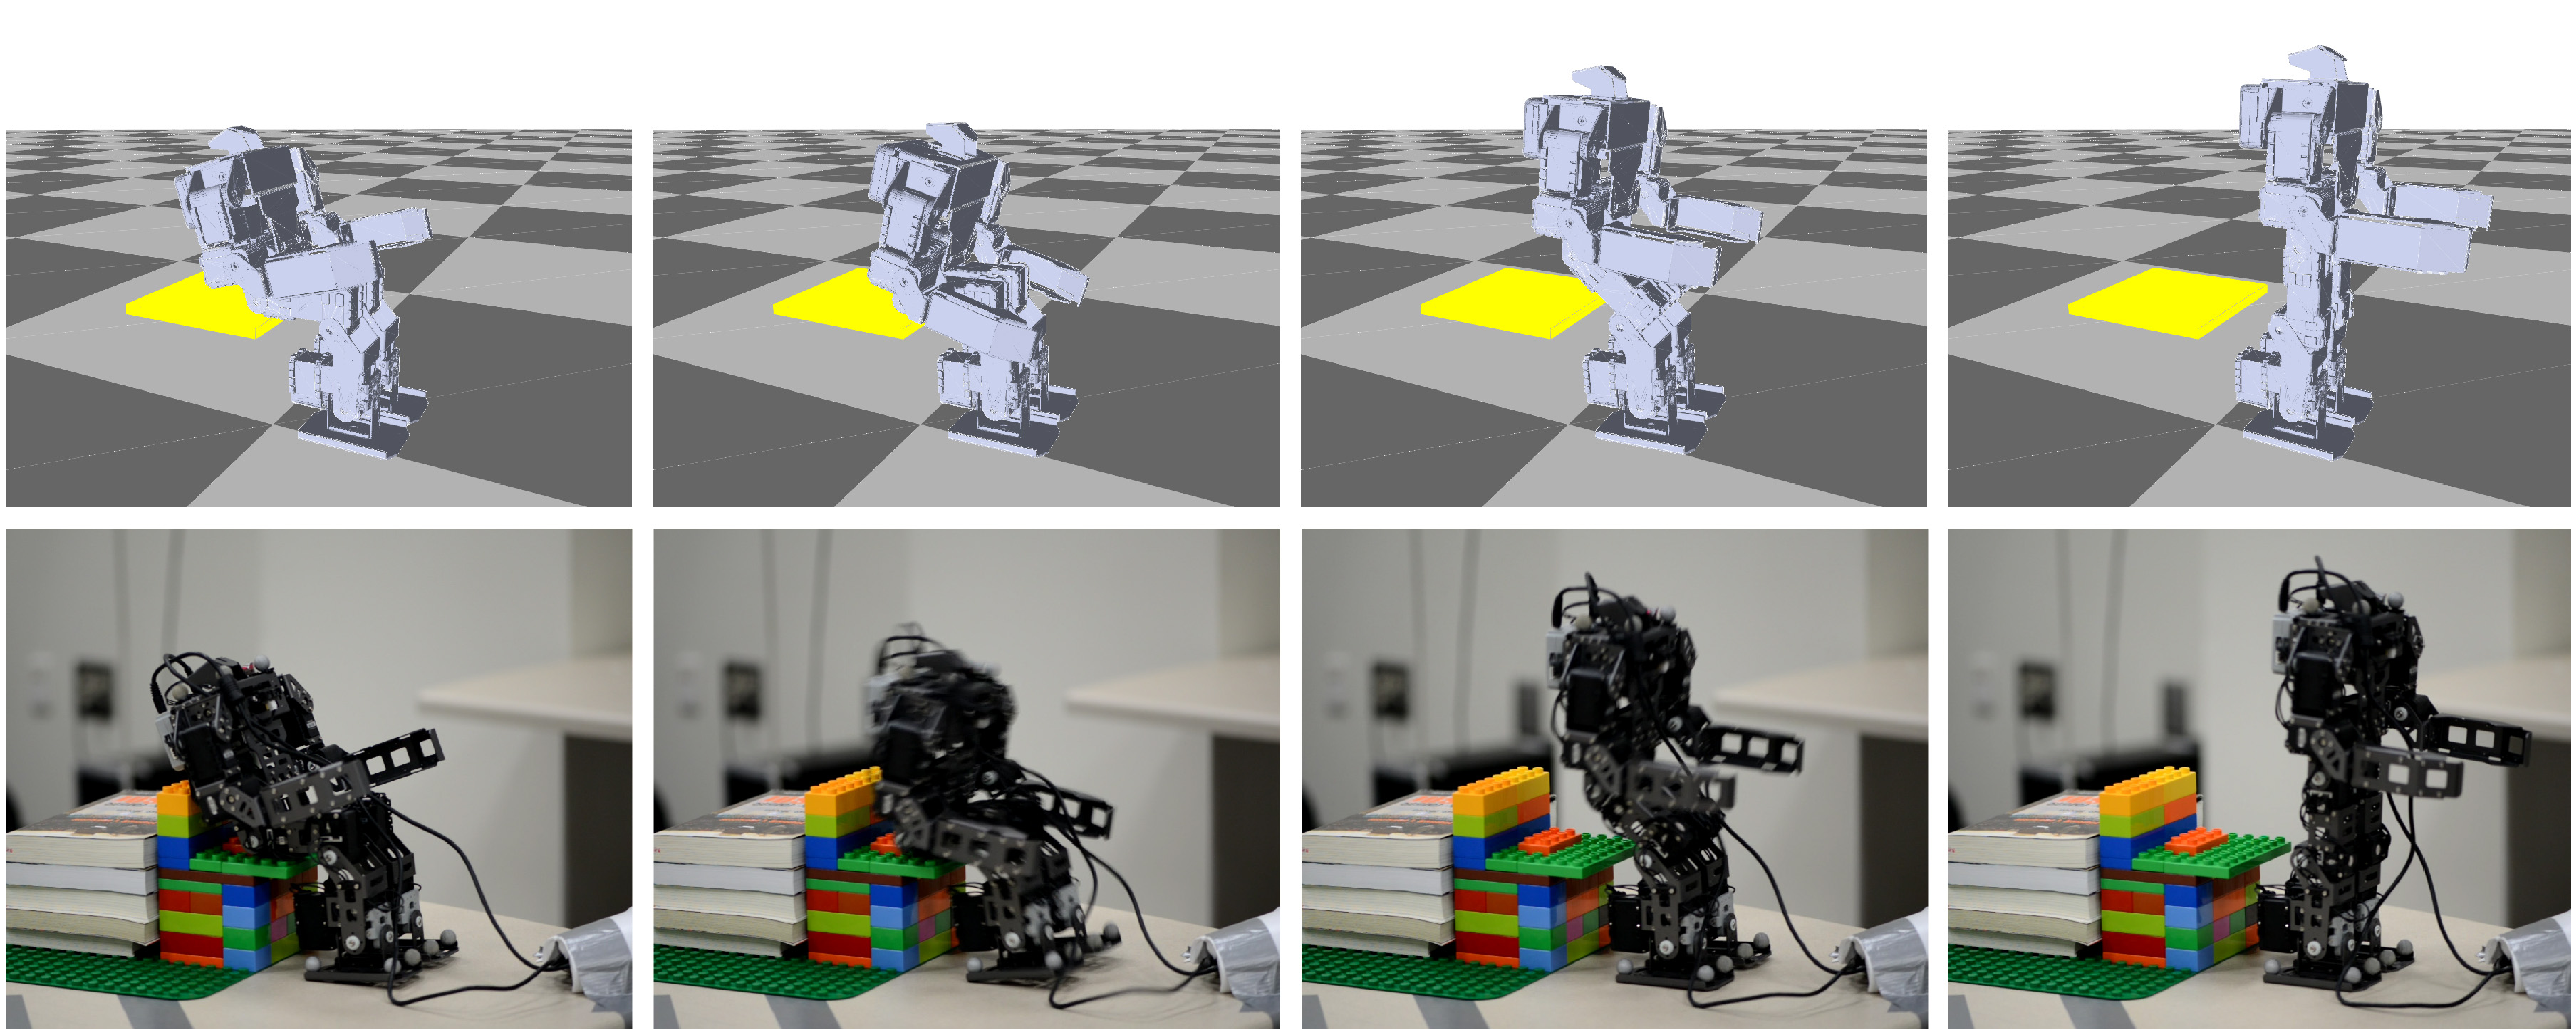
\includegraphics[width=\textwidth]{figures/sit2Stand}
  \caption{The results of the sit-to-stand task in the simulation and on the real robot.}
  \label{fig:sit2Stand}
\end{figure}

The first task that we have tested is to rise from a sitting pose to a standing pose (Figure \ref{fig:sit2Stand}). The initial and final poses $q_0$ and $q_T$ are shown in the leftmost and rightmost images in Figure \ref{fig:sit2Stand}. We parameterize the controller with three keyframes $q_0$, $q_1$ and $q_T$. In addition to $q_0$ and $q_T$ specified by the user, the controller optimization subsystem needs to search for the keyframe $q_1$, and the two time intervals $t_1$ and $t_2$ between the three keyframes. Note that we only change the joint angles of the hips and the knees and keep all other joints motionless throughout the entire motion.

We purposefully choose the initial pose that the legs of the robot extend forward and the projection of the robot's COM in the vertical direction falls far behind the contact points of the feet. If the robot simply extends the hips and the knees to stand up, it will fall backwards. Despite this challenging setup, our system successfully finds a controller that enables the robot to stand up in the simulation. Figure \ref{fig:sit2Stand} shows that the robot first builds up a forward momentum by quickly leaning its upper body to the front. It then starts to extend the hips and the knees at the moment when the COM is approaching the boundary of the support polygon spanned by the feet. This effective standing-up strategy is found automatically by the controller optimization subsystem.

When applying this controller to the real robot, we are surprised to find that it works directly, without the need of simulation calibration. The robot stands up from a chair in the same way as its simulated counterpart does in the virtual world. This shows that the Reality Gap is not always a problem. In some tasks, the stability region of a controller is so large that it can make the discrepancy between the virtual and the real world less critical.

\subsection{Rising from a Leaning Position}

\begin{figure}[!t]
  \centering
  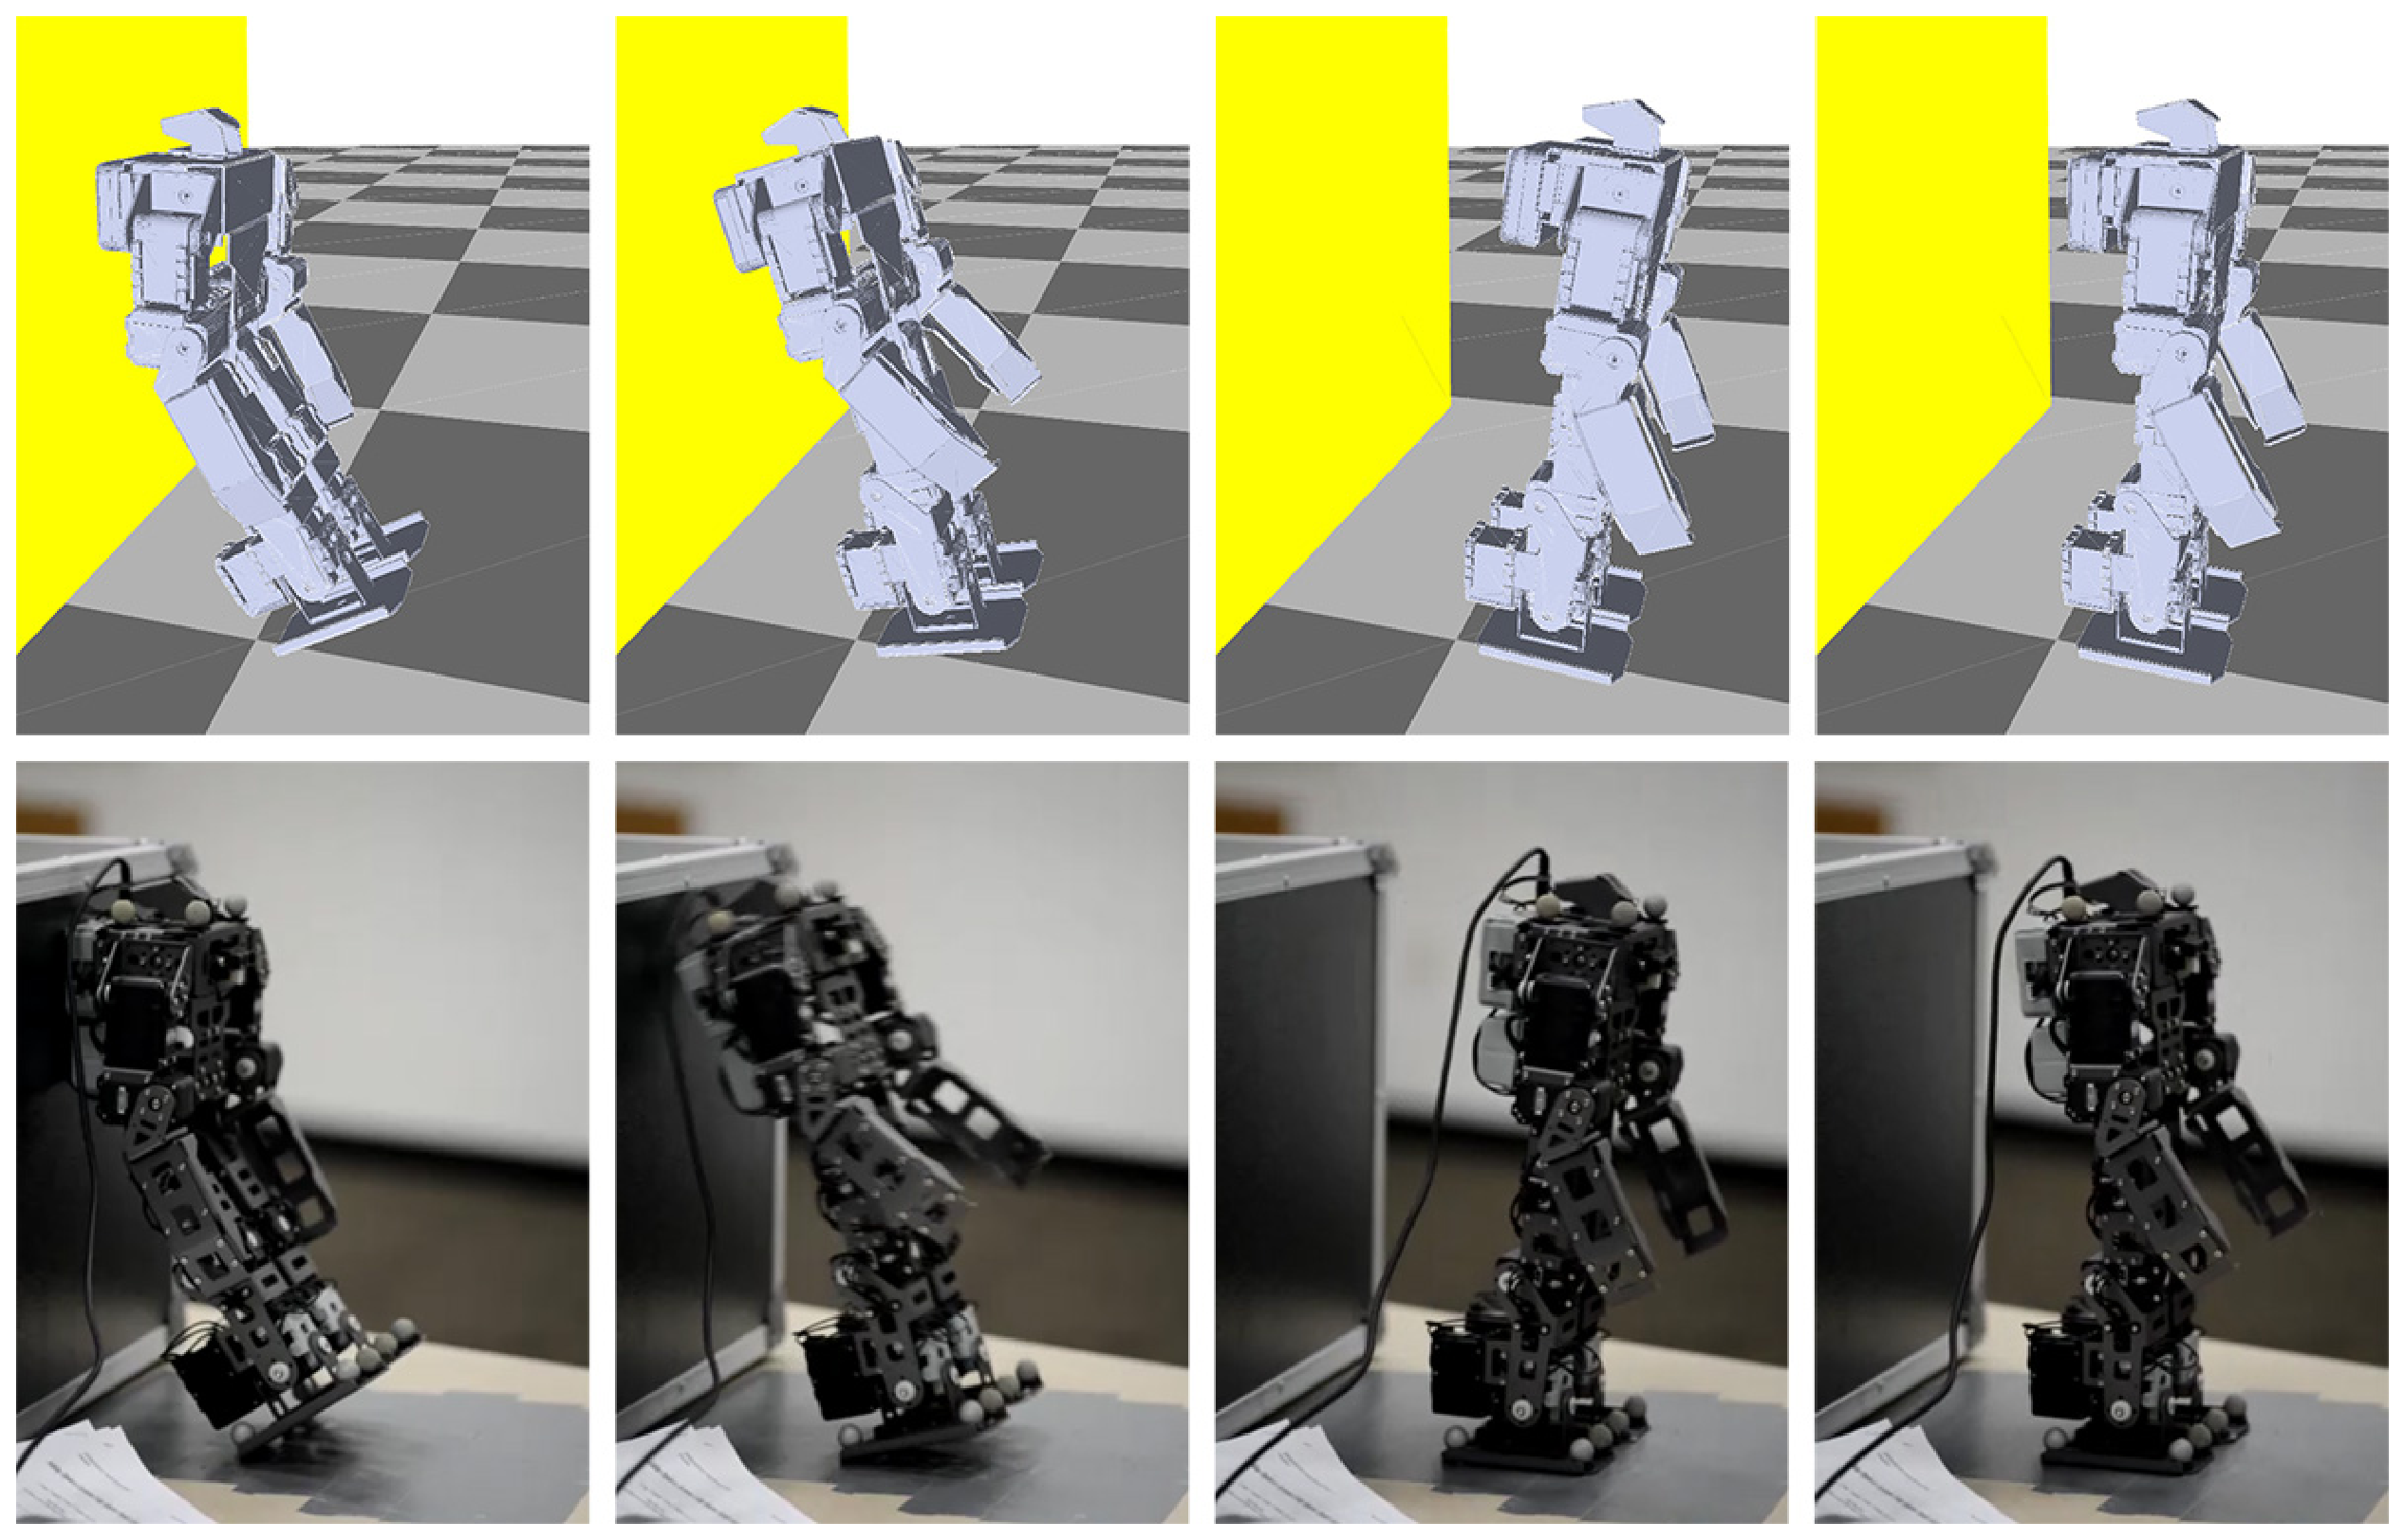
\includegraphics[width=0.7\textwidth]{figures/lean2Stand}
  \caption{The results of the lean-to-stand task in the simulation and on the real robot.}
  \label{fig:lean2Stand}
\end{figure}

In this task, the robot needs to rise from leaning on the wall (the leftmost image in Figure \ref{fig:lean2Stand}) to a standing position (the rightmost image in Figure \ref{fig:lean2Stand}). In the initial configuration, the hip joints are bent and they are straightened out in the final configuration while all other joints do not move. The initial and the final poses are the only two keyframes for this task.

\begin{figure}[!t]
  \centering
  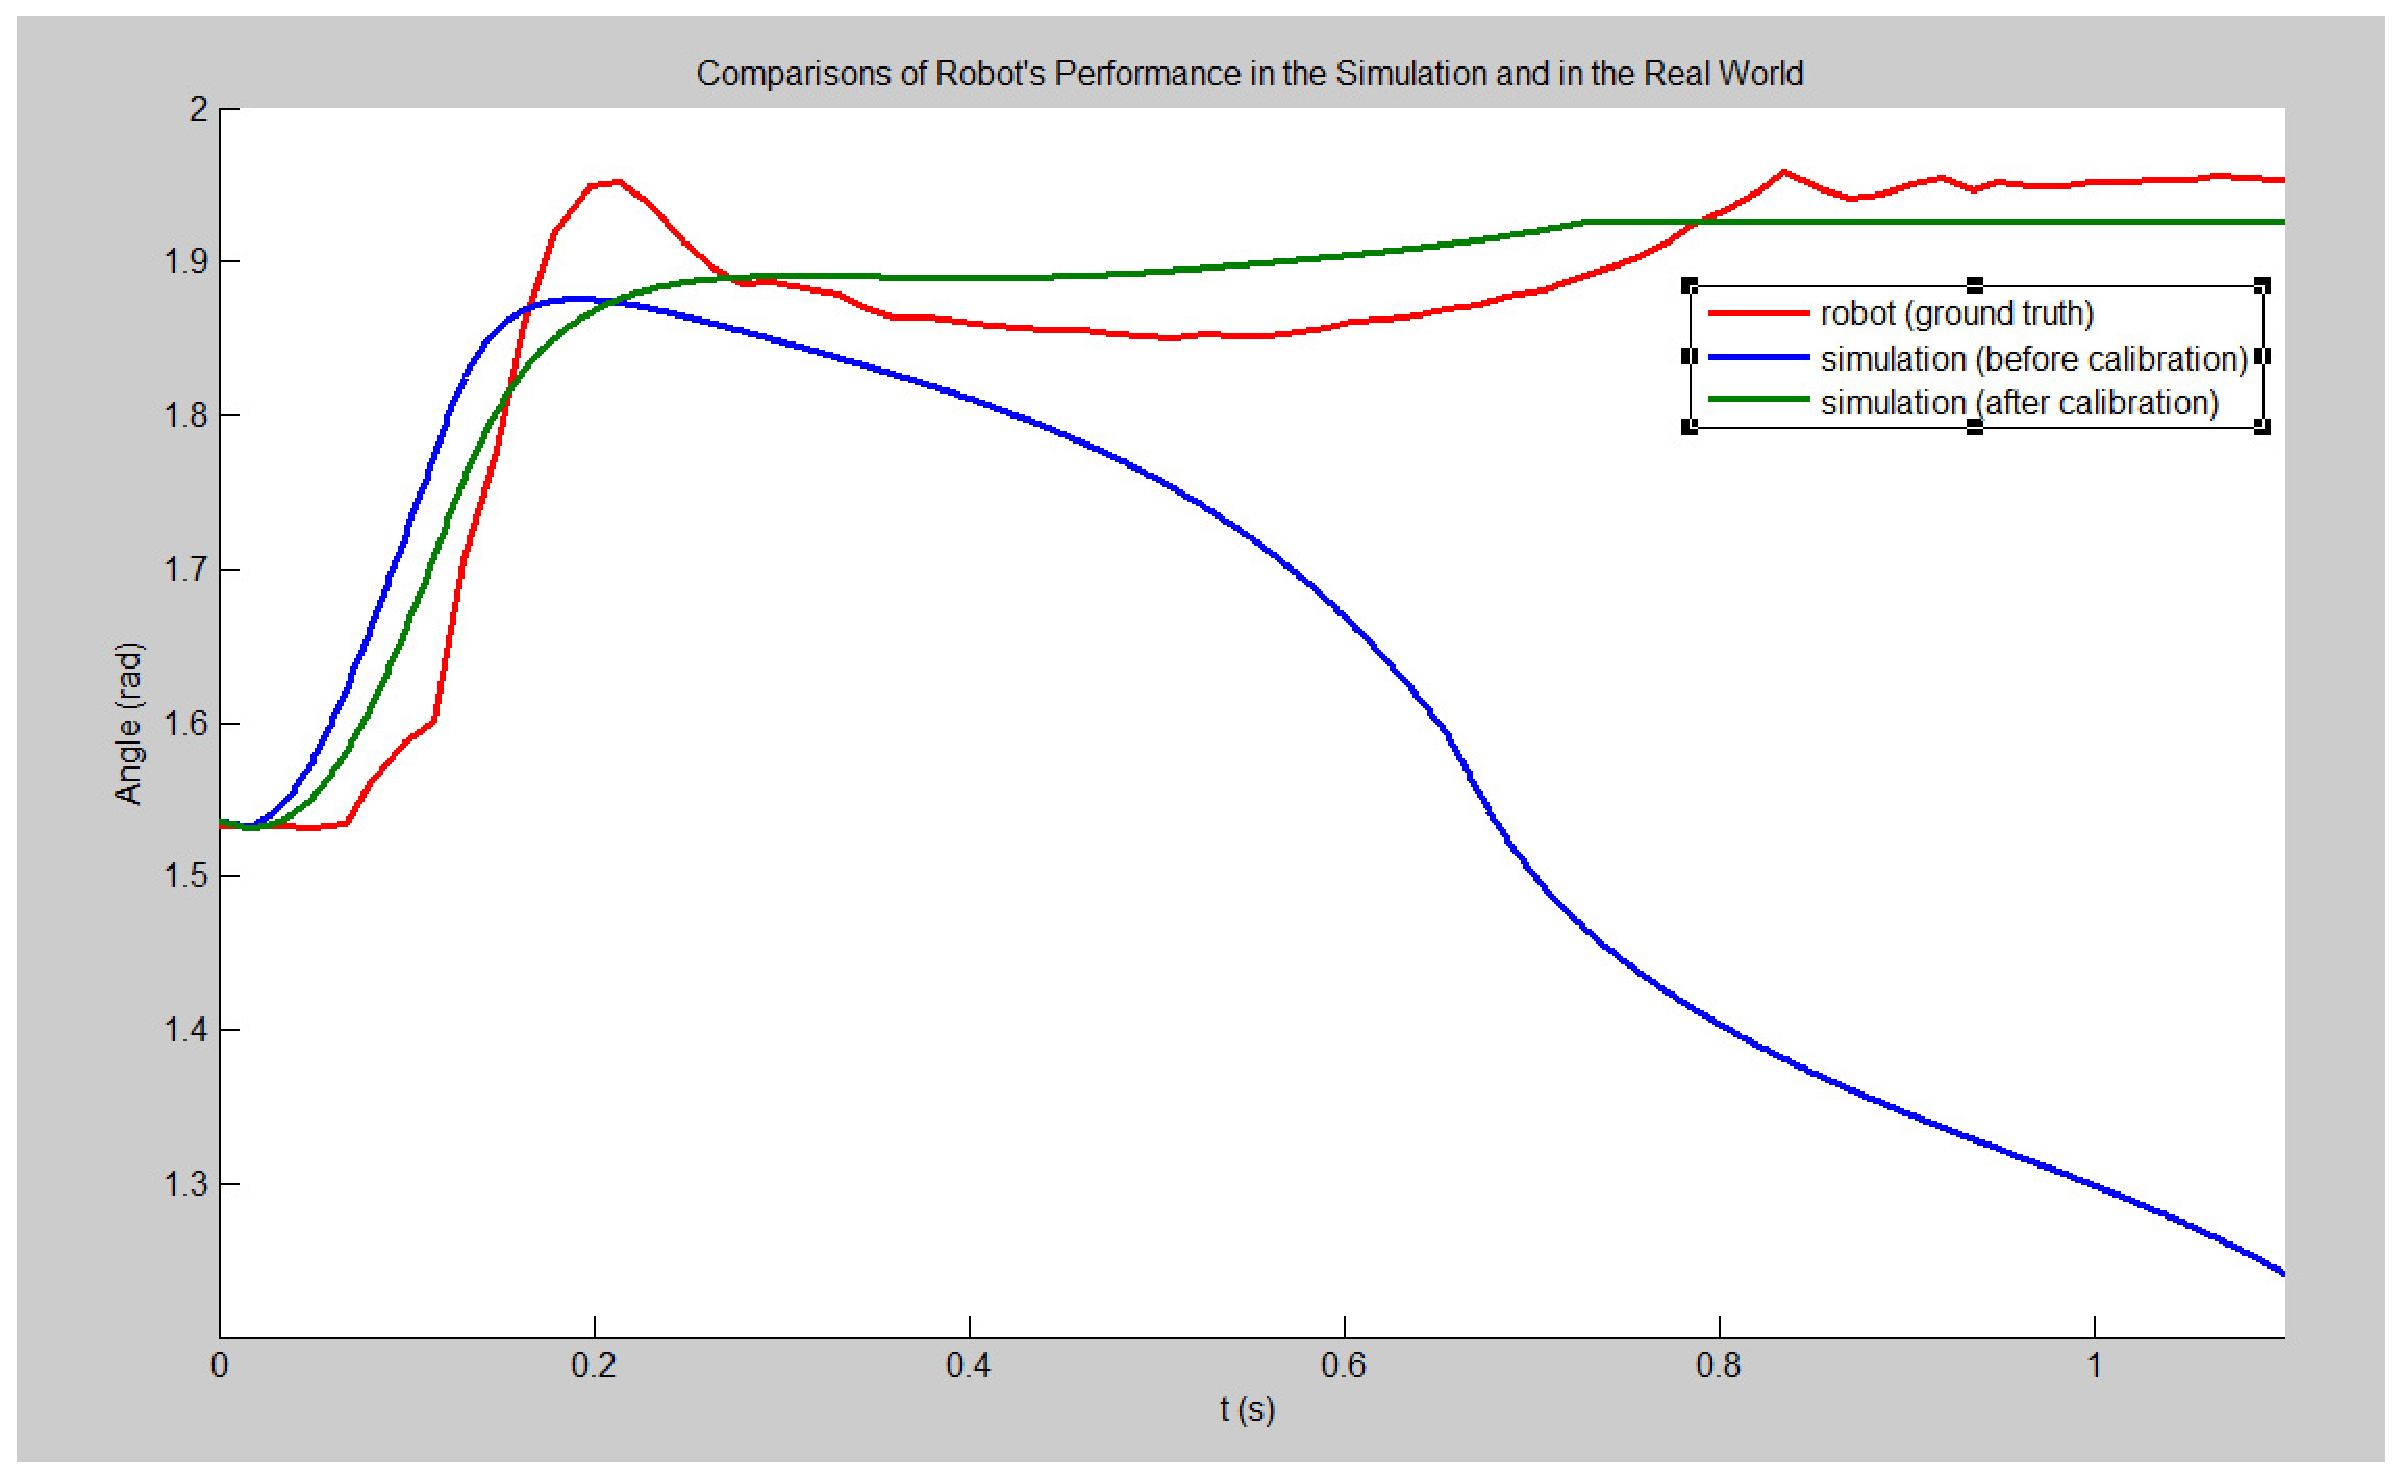
\includegraphics[width=0.7\textwidth]{figures/simRobotCompare}
  \caption{Comparisons of the robot's global orientation over time in the simulation (before/after calibration) and in the real environment.}
  \label{fig:simRobotCompare}
\end{figure}


The goal of controller optimization is to find an appropriate time interval $T$ between these two keyframes. If the time inteval is too long, the robot moves slowly, and cannot accumulate enough momentum to rise up. If this time inteval is too short, the robot move abruptly, which will cause the upper body to bounce off the wall too quickly and fall forward. Without simulation calibration, the optimization cannot find a working controller for this task. The robot cannot rise up when $T\leq 0.10s$ and overshoots when $T > 0.10s$. According to the objective function value, the optimal controller, which still fails the task, uses $T=0.11s$ to move from the initial to the final pose. Using this controller, the robot rises up too quickly and falls forward in the simulation. When we apply this controller to the real robot, we find that its performance in the real world differs drastically from that in the simulation. Rather than falling forward, the robot in the real world cannot rise up. The red and blue curves in Figure \ref{fig:simRobotCompare} show the the trajectories of the robot's global orientation in the simulation and in the real world. After one iteration of simulation calibration, the discrepancy is greatly reduced (Figure \ref{fig:simRobotCompare} green curve). We optimize the controller again in the calibrated simulator. This time, the optimal controller works both in the simulated and in the real environment.

\begin{figure}[!t]
  \centering
  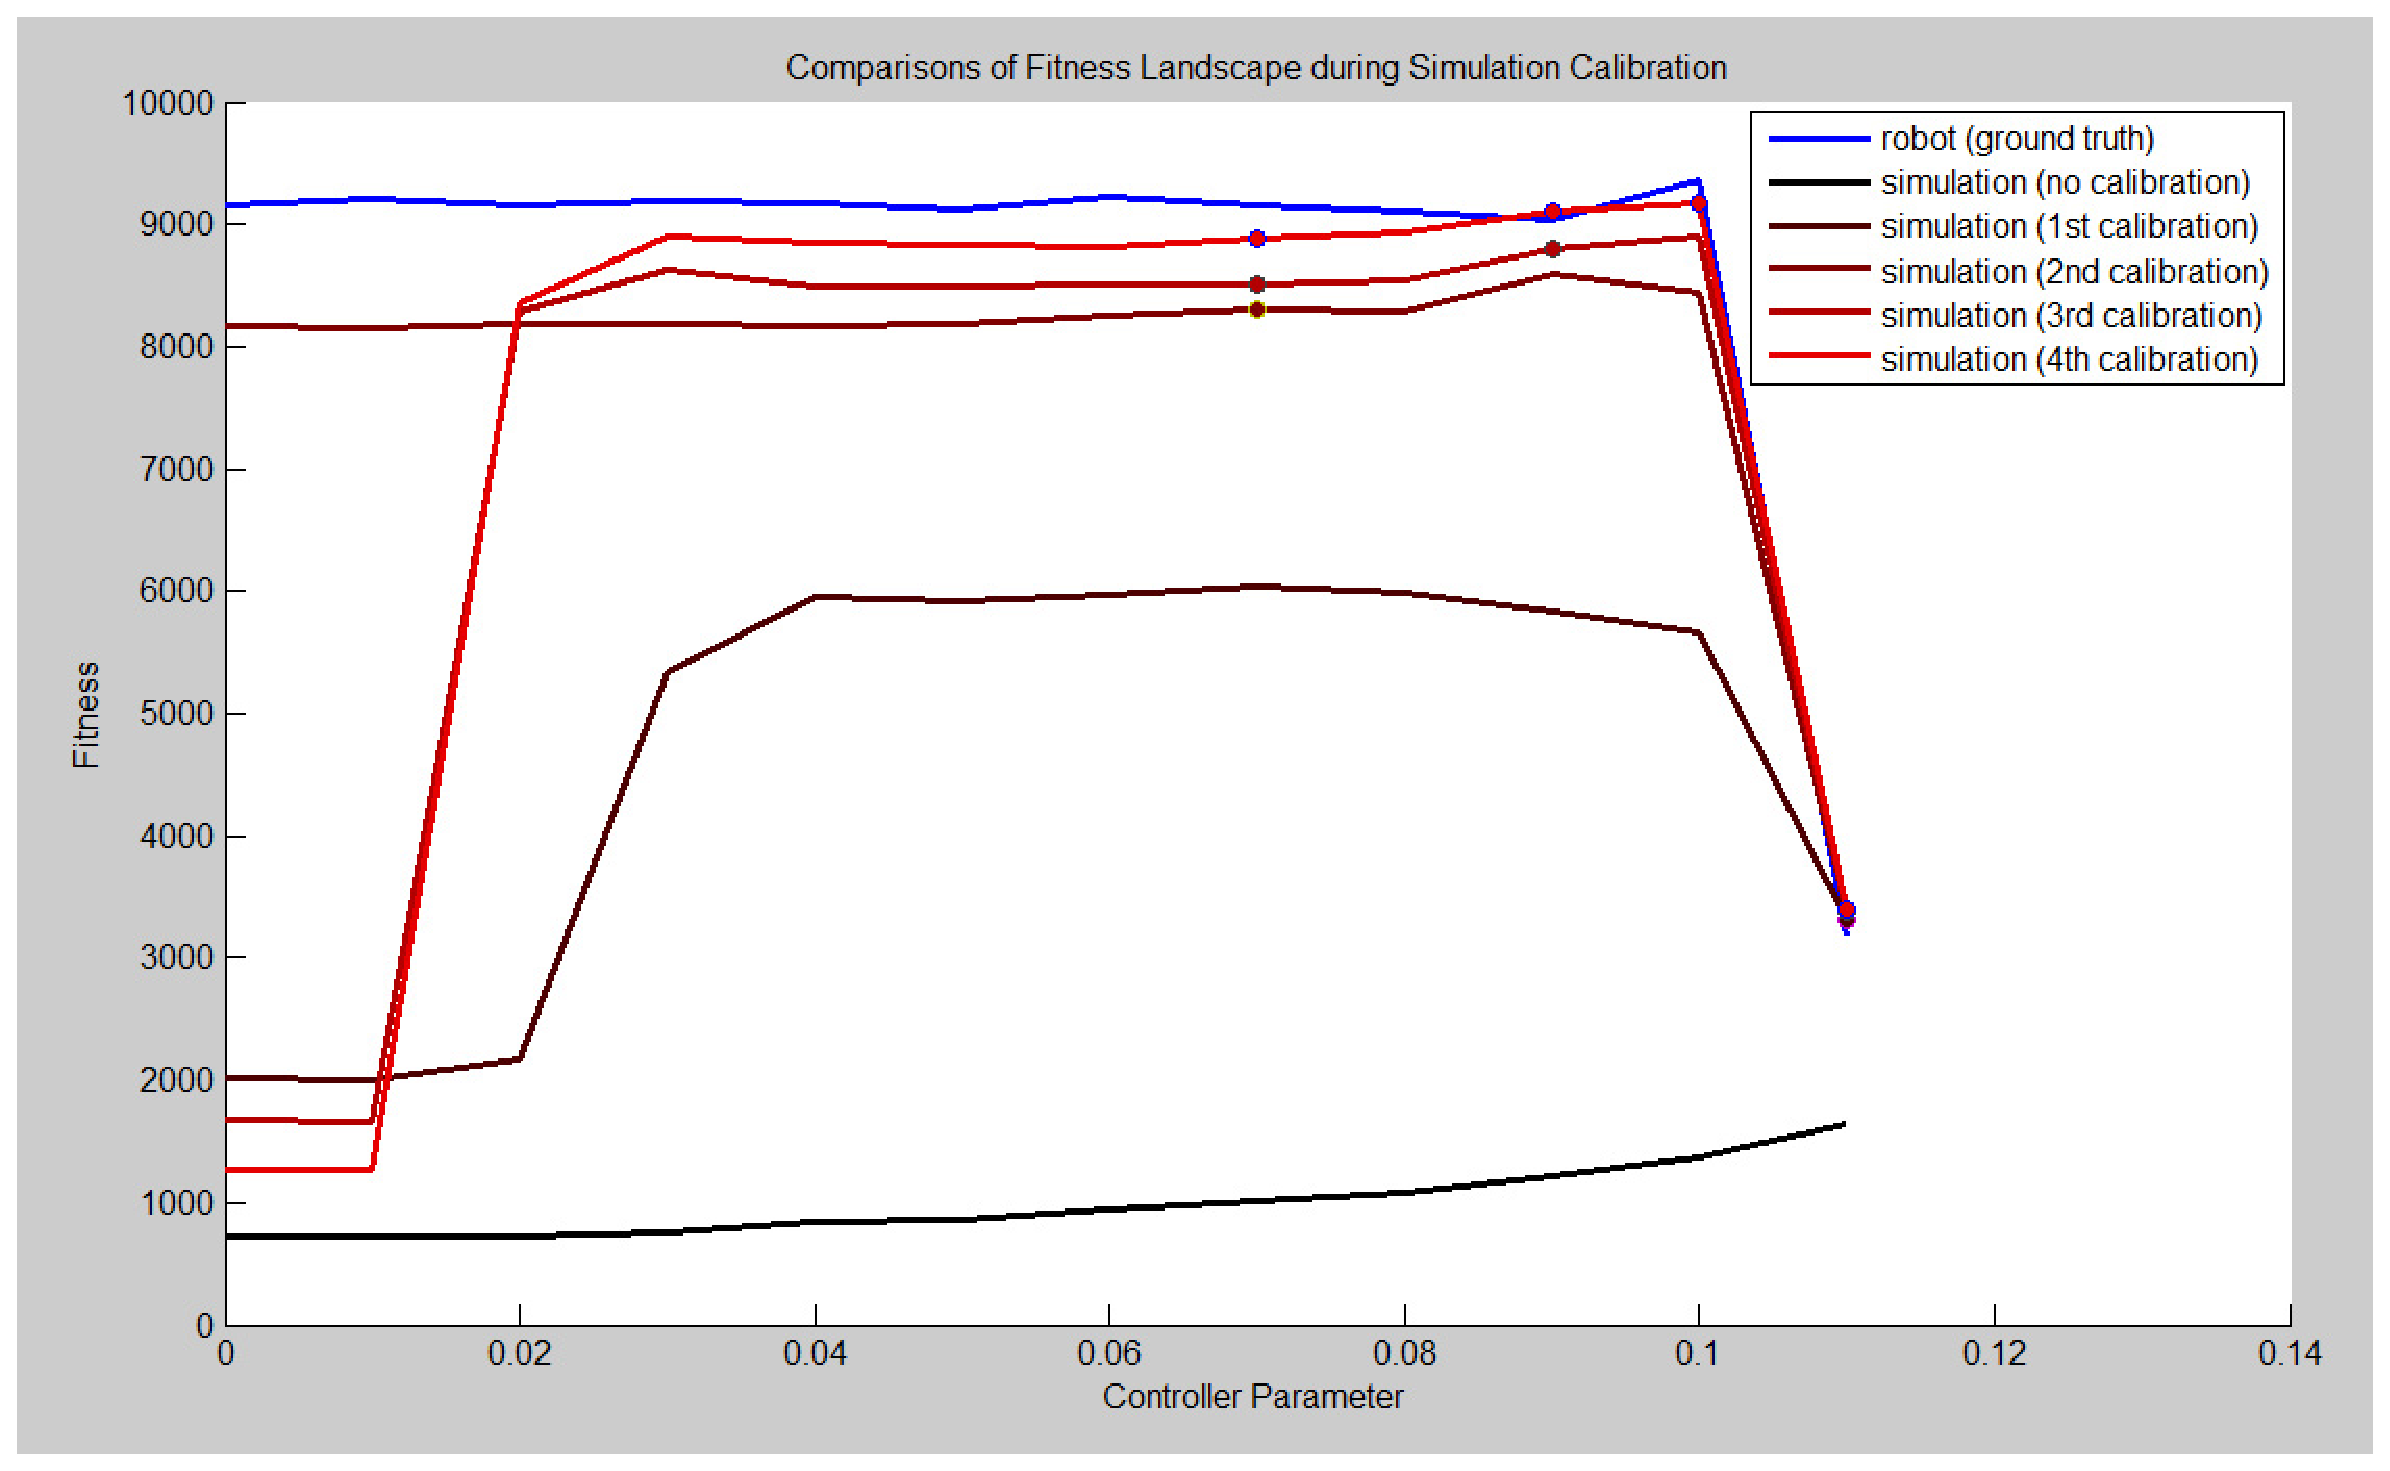
\includegraphics[width=0.7\textwidth]{figures/fitnessLandscape}
  \caption{Comparisons of the fitness functions as more and more iterations of simulation calibration are performed.}
  \label{fig:fitnessLandscape}
\end{figure}

\del{We successfully crosses the Reality Gap using only one iteration of simulation calibration.} \newtext{We are able to transfer the controllers from the simulation to the real environment with only one iteration of simulation calibration.} To better understand how \del{the Reality Gap is gradually narrowed by} simulation calibration \newtext{works} over multiple iterations, we perform an additional evaluation. Figure \ref{fig:fitnessLandscape} shows the fitness functions after different number of iterations of simulation calibration. The blue curve is the fitness function on the real robot by varying the control parameter $T$ in the range of $[0, 0.11]$. It serves as the ground truth. The fitness function stays at a high value when $T\in[0, 0.1]$, which means that the real robot can successfully rise if the controller uses less than 0.1s to change the pose from the initial to the final configuration. In contrast, without simulation calibration, the fitness function (lowest black curve) stays at a low value for the entire control space. In other words, no controller exists that can make the robot stand up in the simulation. The gap between the blue and the black curves is analogue to the Reality Gap. One iteration of system calibration brings the fitness function in the simulation towards the ground truth. As more iterations are performed, the fitness function in the simulation (brown and red curves) gradually approaches the ground truth, and the Reality Gap is narrowed in this process. Note that a large discrepancy still exists in the region of the parameter space where $T<0.02s$. This is probably caused by two reasons. First, in the region of $T<0.02s$, the torque output of the servo is at its limit but the torque limit is not considered in simulation calibration. Second, the controllers and the data (the red circles in Figure \ref{fig:fitnessLandscape}) that we use in simulation calibration concentrate on the right half of the parameter space, which makes it difficult to generalize to a region where the data is scarce ($T<0.02$). However, this could be beneficial in many applications because the computational resource is focused at the important regions near the successful controllers.

\subsection{Rising from a Kneeling Position}

\begin{figure}[!t]
  \centering
  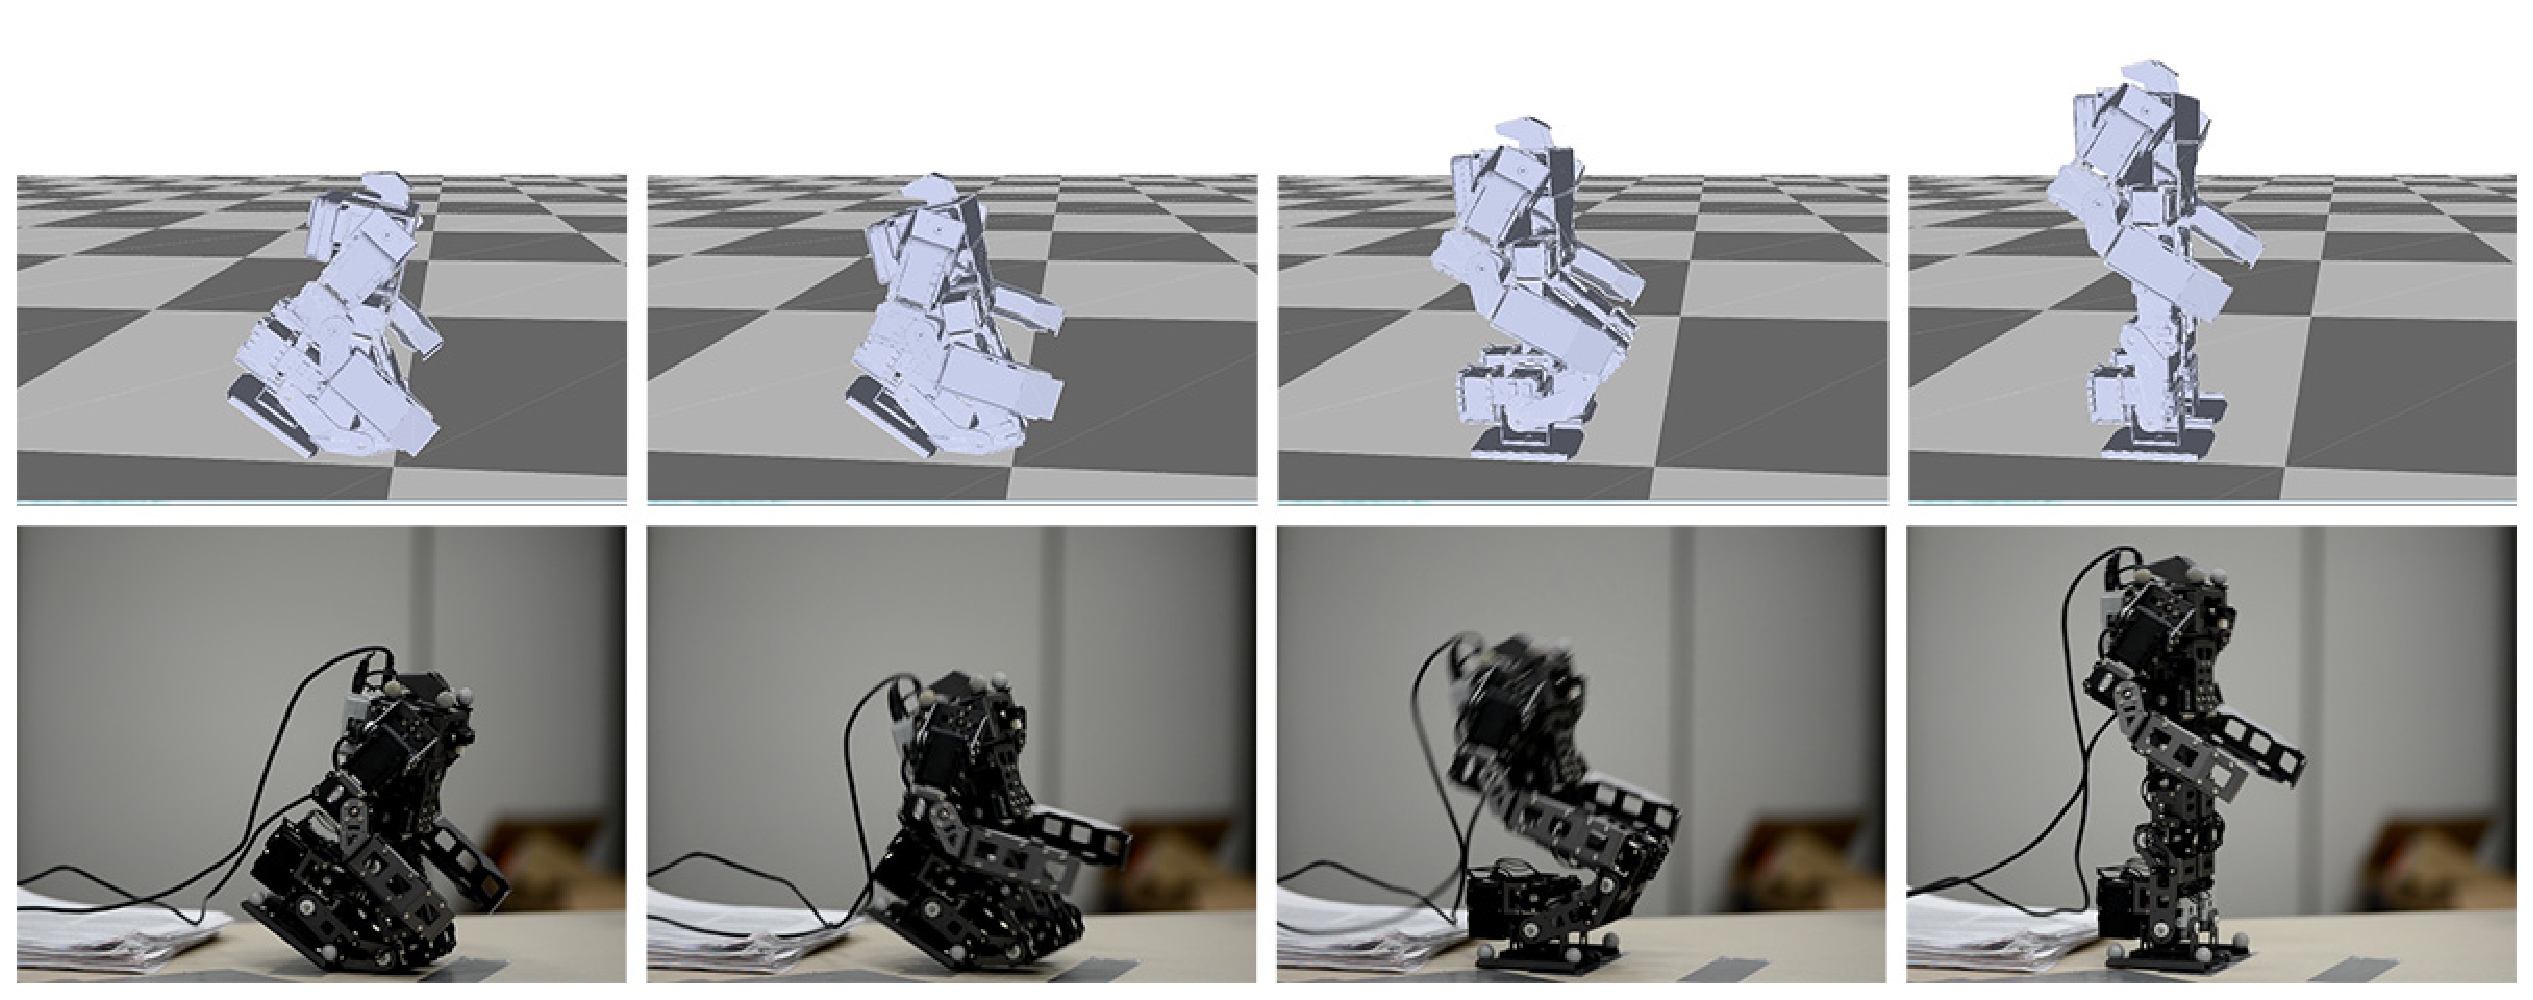
\includegraphics[width=\textwidth]{figures/kneel2Stand}
  \caption{The results of the kneel-to-stand task in the simulation and on the real robot.}
  \label{fig:kneel2Stand}
\end{figure}

Figure \ref{fig:kneel2Stand} shows that the robot stands up from a kneeling pose. Between the user-specified initial and final poses, the controller consists of two additional keyframes. The optimization needs to search for these keyframes and the time intervals between adjacent keyframes. Similar to other examples, we only allow the joints on the lower body of the robot to move. The controller optimized in the simulation demonstrates an agile getting-up motion: The robot first leans its upper-body backwards. As its COM is moving to the back, it quickly bends the hip, flexes its ankles and stands up. This entire motion resembles one of the most agile ways that we human get up from a kneeling position when we do not use our hands for additional support. Although this controller works perfectly in the simulation, the robot falls backward in the real world. After simulation calibration, the performance of the simulated robot comes closer to the real world scenario: The robot also falls backward in the simulation. Using the calibrated simulator, we optimize a new controller, with which the robot can successfully stand up from the kneeling position in the real world (Figure \ref{fig:kneel2Stand}).


\subsection{Flipping to a Handstand Position}


\begin{figure}[!t]
  \centering
  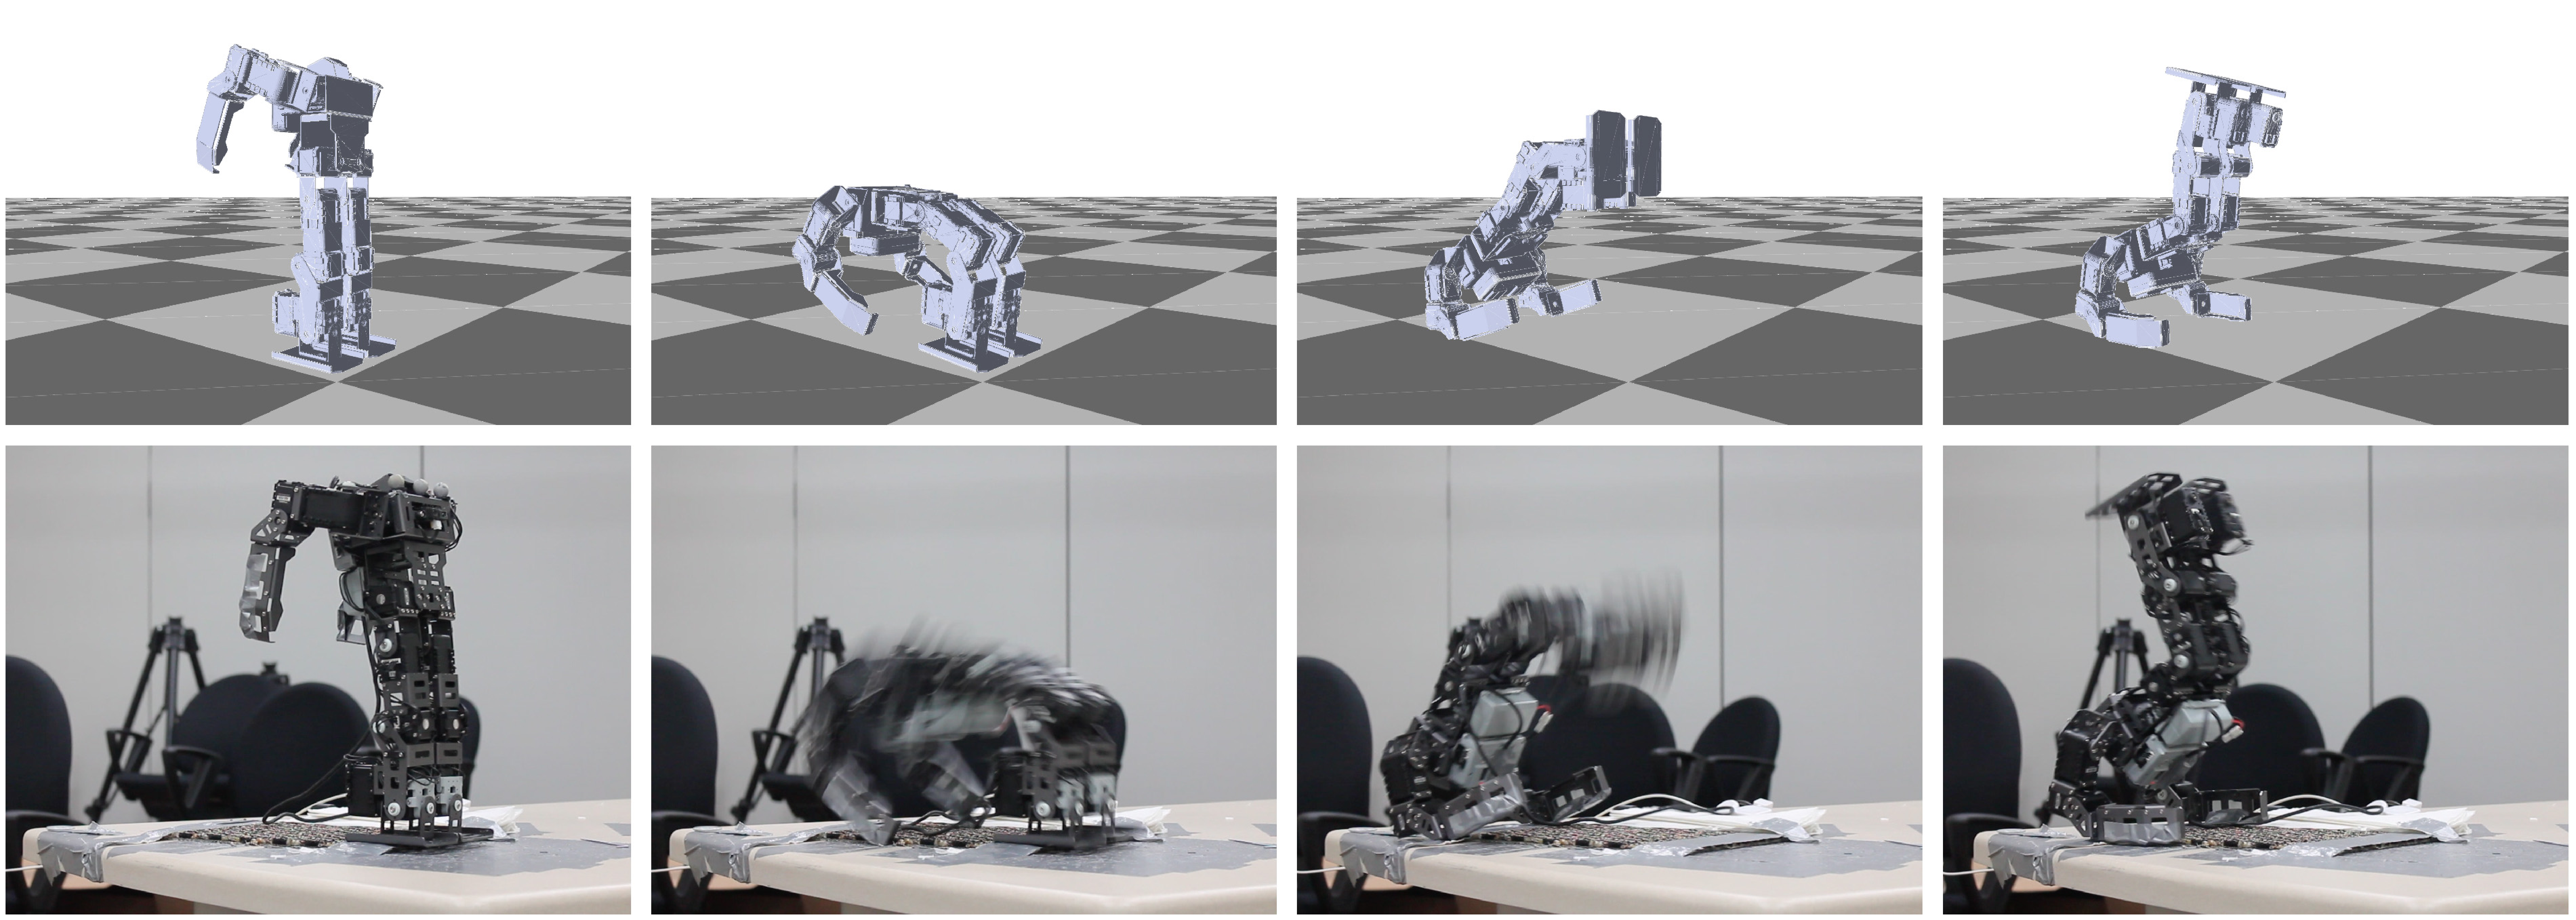
\includegraphics[width=\textwidth]{figures/stand2Hand}
  \caption{The results of the stand-to-handstand task in the simulation and on the real robot.}
  \label{fig:stand2Hand}
\end{figure}

We test our system with a challenging gymnastic action: flipping to a handstand position from a standing pose (Figure~\ref{fig:stand2Hand}). There are two unique challenges in this task. First, the speed and the curvature of the initial arching motion is crucial and only a narrow range of such speed and curvature can lead to a balanced handstand. Second, the USB cable that connects the robot to the computer will inevitably hit the ground during the backflip, which injects a strong perturbation that is not modeled in our simulation.

With two iterations of simulation calibration and controller optimization, our system finds a successful controller that works both in the simulation and in the real world: The robot arches back rapidly and lifts its feet after the arms touch the ground. It shows that our system can automatically design controllers for challenging locomotion tasks, even with strong unmodeled perturbations.


\section{Discussion}

This chapter has presented an end-to-end solution to automatically design locomotion controllers for robots. This solution consists of a set of computational tools: a simulation tool that simulates the dynamics of the robot and its environment, an optimization tool that automatically searches for a controller in the virtual environment and a calibration tool that improves the simulation accuracy to ease controller transfer from the virtual to the real world. This powerful system allows us to efficiently design controllers of a humanoid robot to achieve four different tasks, rising from leaning, sitting and kneeling poses to an erect stance, and flipping from a standing to a handstanding pose.

Since the main goal of this work is to demonstrate that the computational tools developed for character animation, including physical simulation and controller optimization, can be applied to robotics, the biggest challenge is \del{the Reality Gap. The evaluation shows that our simulation calibration algorithm is effective to narrow down this gap.} \newtext{ to transfer the controllers developed in the simulation to the real environments. In all the examples, at most two iterations of calibration is needed before we can successfully transfer the controller to the real robot. However, we want to emphasize that the goal of simulation calibration is not to find the true simulation parameters. Instead, it finds a set of parameters that reduce the discrepancy between the simulation and the real experiment for a specific locomotion task. We observe that the simulation parameters optimized for the task of lean-to-stand can be different from those of kneel-to-stand. In other words, the calibrated simulator is only valid for the current task and should not be used in a different task. It would be more interesting if simulation calibration can discover the true parameter value so that the calibrated simulator can be used for different tasks. We believe that this is possible if we use controllers and their corresponding robot performance data from multiple different tasks as the input of simulation calibration.} \del{If the tasks are the same but the initial configurations are slightly different, the result of simulation calibration can be reused. For example, in the task of lean-to-stand, we can use a simulator calibrated for a specific initial leaning angle to optimize controllers if the robot needs to stand up from a different initial leaning angle. In this case, our experiments show that the result of simulation calibration can be reused if the initial leaning angle is perturbed within five degrees. }

\newtext{Crossing the Reality Gap is important for robotics because it can truly unleash the power of the computational tools and fundamentally change how robot controllers will be designed. Due to the variety and complexity of the causes of the Reality Gap, crossing it is an extremely challenging research problem. Our work only scratches the surface of this problem. A lot of future research need to be conducted in this area. For example, our locomotion tasks are relatively short, simple and do not require feedback controllers. We plan to extend our algorithm to more difficult tasks, such as walking and running.} In our examples, we have shown that adjusting the COM and the actuator gains are enough, but other simulation parameters might also be important for a wider range of tasks. Including more simulation parameters and performing feature selection would be a promising direction for future work. In addition, some discrepancies between the simulation and the real world may not be explained by inaccurate simulation parameters alone. Unmodeled dynamics could also contribute to the discrepancy. Combining parametric and non-parametric models in simulation calibration for unmodeled dynamics is also an interesting avenue for future work.


